%\documentclass[handout]{beamer}
\documentclass{beamer}

\begin{document}
	\title{Sieve of Eratosthenes}
	\author{Martin Pola}
	\date{\today}

    \frame
    {
        \frametitle{Sieve of Eratosthenes}

        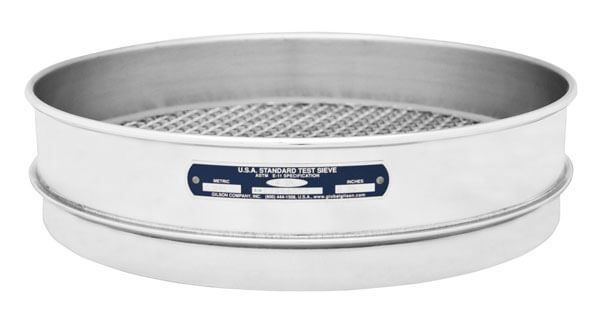
\includegraphics[width=\textwidth]{sieves.jpg}
    }
    
    \frame
    {
        \frametitle{Idea}

        \begin{block}{Initial assumption}
           All numbers are prime numbers.
        \end{block}

        \vspace{0.5cm}
        
        \begin{enumerate}
            \item Start at the prime number 2
            \item Keep the prime number, but remove all multiples
            \item Move to the next prime number -- repeat from step 1
        \end{enumerate}
    }
    
    \frame
    {
        \frametitle{Coding steps}
        
        \begin{itemize}
            \item Define a constant max number
            \item Create an array to keep track of prime numbers and composite numbers
            \item Mark all numbers as prime numbers
            \item Outer \texttt{for} loop for current number, inner \texttt{for} loop for multiples
            \item Go through the array and print only prime numbers
        \end{itemize}
    }
\end{document}